\chapter{Preparation}
\label{chap:preparation}
After identifying the main goals, these coarse requirements are refined to be precise about objectives, and to drive development.
This results in a set of \emph{requirements} that can be analysed to predict problems and measure success.
Once any problems are resolved, work can begin on implementation.
Some mathematics is required to increase precision, and can be used to direct refinement of requirements.
In this chapter I discuss the theory required to begin formalisation, briefly introduce Isabelle, and produce a list of requirements.

\section{\(\lambda\)-Calculus}
\label{sec:lambda-intro}
The \(\lambda\)-calculus~\cite{lambda-overview} is a system of computation, represented by operations on \emph{terms}.
\begin{definition}
Terms \(M\) are inductively defined:
\begin{enumerate}
\item
A variable, \(x\), is always a term.
These may be sub-categorised to be \emph{bound} if some \emph{binder} in an expression binds them, or \emph{free}, if there is no such binder.
\item
If \(M\) is a term, abstractions \(\lambda x.M\) are also terms.
This intuitively represents an anonymous function returning \(M(x)\)), and \emph{binds} \(x\) in \(M\).
\item
If \(M\) and \(N\) are terms, applying \(M\) to \(N\) is also a term, \(\wrap{M\ N}\).
\end{enumerate}
\end{definition}

\noindent
Terms can be represented with an algebraic datatype.
For instance, in Standard ML:
\begin{minted}{SML}
datatype 'a trm =
    Var of 'a
  | Fn  of ('a * 'a trm)
  | App of ('a trm * 'a trm)
\end{minted}

Computation here is performed by \(\beta\)-reduction: terms \emph{reduce} to another term according to a series of rules, and hence computation occurs by sequential reductions.

\begin{definition}
\(M \to_\beta M'\) when one of the following holds:
\begin{enumerate}
\item
If left or right subterms of an application reduce, then the application also reduces: if \(M \to_\beta M'\), then \(\wrap{M\ N} \to_\beta \wrap{M'\ N}\).
\item
If \(M \to_\beta M'\), then \(\lambda x.M\) becomes \(\lambda x.M'\).
\item
If a term is of the form \(\wrap{\wrap{\lambda x.M}\ N}\), then it is a \(\beta\)-redex, and reduces to
\[
M[x := N]
\]
(\emph{viz.} \(M\) with occurrences of \(x\) substituted in a capture-avoiding fashion for \(N\)).
\end{enumerate}
\end{definition}

The order in which reduction steps occur in a computation is important for many applications of the \(\lambda\)-calculus, but I did not use this property in my dissertation.
Substitution, used informally above, is defined recursively.

\begin{definition}
Suppose \(N\) is substituted for \(x\) in \(M\), and \(y\) is any name that is not \(x\).
Then the result, \(M[x := N]\), is
\[
M[x := N] =
\begin{cases}
N & M = x\\
M & M = y\\
M & M = \lambda x. M'\\
\lambda y. \wrap{M'[x := N]} & M = \lambda y. M'\\
\wrap{M_1[x := N]\  M_2[x := N]} & M = \wrap{M_1\ M_2}\\
\end{cases}
\]
\end{definition}

\(\beta\)-reduction has \emph{confluence} property.
Confluence states that if \(A\) reduces in many steps to \(B\), and similarly on another path to \(C\), there is a \(D\) such that \(B\) and \(C\) reduce to \(D\), asserting that the order of reductions does not affect the final result.
There are terms that cannot be further reduced, like \(x\), \(\lambda y.y\), or \(\wrap{f\ x}\).
These terms are considered to be values, or \emph{in normal form}.

\begin{definition}
Variables \(x\) are in normal form.
Applications are in normal form if they are not a \(\beta\)-redex and both subterms are themselves in normal form.
Binders are in normal form if their bound subterm is in normal form.
\end{definition}

\section{Simple types}
\label{sec:type-intro}
Untyped calculi have disadvantages.
No types mean that unexpected constructions can occur, such as applying a non-function, which a type system generally prevents.
``Programs'' in the calculus may also fail to terminate: a sequence of reductions may not necessarily finish.
Consider

\[
\Omega = \wrap{\lambda x. \wrap{x\ x}}\ \wrap{\lambda x. \wrap{x\ x}}
\]

Then the only possible reduction for \(\Omega\) produces \(\Omega\), which may not terminate.
The untyped calculus can be extended to include a type system while maintaining an approach to names: a \emph{type} is simply added to each binder, so \(\lambda x.M\) becomes \(\lambda (x:T).M\), for an arbitrary \(T\).
Note that I use this, the Church style of typing, exclusively in my project.

\begin{definition}
Simple types \(\tau\) are either
\begin{enumerate}
\item
A base type, say \(\iota\).
\item
An arrow type \(\tau_1 \to \tau_2\) from one type to another.
\end{enumerate}
\end{definition}

Adding simple types to the binders of the untyped calculus produces the \emph{simply-typed} \(\lambda\)-calculus.
The typing relation \(\Gamma \vdash M : \tau\) is given inductively in Figure \ref{fig:typing}.
\(\Gamma\) here is a typing context: a partial function from variables to types.

\begin{figure}
\begin{mathpar}
\inferrule[var]
 {\Gamma(x) = \tau}
 {\Gamma \vdash x : \tau}

\inferrule[fn]
 {\Gamma\{x \mapsto \tau\} \vdash M : \sigma}
 {\Gamma \vdash \lambda (x : \tau). M : \tau \to \sigma}

\inferrule[app]
 {\Gamma \vdash M : \tau \to \sigma \\ \Gamma \vdash N : \tau}
 {\Gamma \vdash \wrap{M\ N} : \sigma}
\end{mathpar}
\caption{typing rules for the simply-typed calculus}
\label{fig:typing}
\end{figure}

I show several correctness properties that are not possible in an untyped calculus: progress, type preservation (subject reduction), and safety.
These capture semantics of Milner's~\cite{milner} maxim ``well-typed programs do not go wrong''.

\begin{definition}
The progress property asserts if \(\Gamma \vdash M : \tau\), \(M\) is either in normal form or can be reduced further.
\end{definition}

\begin{definition}
The preservation property holds if, assuming \(\Gamma \vdash M : \tau\) and \(M\) reduces to \(M'\), \(\Gamma \vdash M' : \tau\).
\end{definition}

Generally these are desirable properties: expressions should not ``get stuck'' computing non-values, or change type mid-reduction.

\begin{definition}
A language has the safety property if, when reducing a well-typed term \(M\) by a number of steps resulting in \(M'\), \(M'\) is either in normal form, or can be reduced further.
\end{definition}

This property is the main goal of verification: it shows that if a term is well-typed, there is no scenario in which reduction fails --- the term reduces, or computation has finished.

\begin{center}
\rule{.3\textwidth}{.5pt}
\end{center}

Type inference is the process of producing a type \(\tau\) for \(M\) such that \(\Gamma \vdash M : \tau\).
One advantage of the simply-typed calculus is that type inference is decidable, and straightforward, with no unification steps (in the Church style) or complexity that more advanced typing systems encounter.
The type inference algorithm \(\infertype(\Gamma, M)\) can be described by
\[
\infertype\wrap{\Gamma, M} =
\begin{cases}
\Gamma(x) & M = x\\
\tau \to \infertype\wrap{\Gamma\{x \mapsto \tau\}, N} & M = \lambda (x : \tau). N\\
\mathrm{apply}\wrap{\infertype\wrap{\Gamma, A}, \infertype\wrap{\Gamma, B}} & M = \wrap{A\ B}
\end{cases}
\]
where \(\mathrm{apply}\wrap{\tau \to \sigma, \tau}\) produces \(\sigma\).
All other input is undefined.
I use an option type to propagate errors upwards, which the above omits for simplicity.
Type inference can be shown correct with respect to a type system if it exclusively infers correct types (\emph{soundness}), and infers all possible correct types (\emph{completeness}).
With these properties, the typing rules and the inference algorithm are equivalent.

\section{The problem of \(\alpha\)-equivalence}
\label{sec:alpha-equivalence}
This representation, with names and binders, is insufficient.
It is convenient to reason that e.g. \(\lambda x.x\) and \(\lambda y.y\) are equal: they produce identical results on all inputs.
However, they differ structurally: \(x\) is not the same as \(y\).
This reasoning is called \emph{\(\alpha\)-equivalence}.

\begin{definition}
The \(\alpha\)-equivalence relation \(\equiv_\alpha\) is the least congruence on terms such that
\[
\lambda x.M \equiv_\alpha \lambda y.M'
\]
where y does not occur free in \(M\), and \(M'\) is \(M\) with \(x\) substituted for \(y\) (avoiding captures).
\end{definition}

Such an equivalence could be assumed whenever required.
Nonetheless, it is cumbersome to carry such an assumption, and proof assistants often reason better about equality than equivalence relations, as automation tools are tuned for equality.
This problem can be solved using \emph{quotient types}~\cite{quotient}.

\begin{definition}
A quotient type \(Q\) is a base type \(R\), an equivalence relation \(\sim\) on \(R\), and functions \(\mathrm{Abs} : R \to Q\) and \(\mathrm{Rep} : Q \to R\).
Items \(q_1 : Q\) and \(q_2 : Q\) are equal iff \(Rep\ q_1 \sim Rep\ q_2\).
\end{definition}

I now define a quotient type for \(\lambda\)-terms modulo \(\alpha\)-equivalence by encoding a datatype for pre-terms without equivalence as before, then the new type is a quotient over \(\alpha\)-equivalence.
While we now use equality directly, this equivalence relation is awkward to use.
There are alternative ways of handling names, the most prominent de Bruijn indices~\cite{deBruijn}, Higher-Order Abstract Syntax~\cite{HOAS} (HOAS), and nominal techniques~\cite{nominal}.
Ideally, these would allow the ``Barendregt convention'' for reasoning about names: for any term, assume that the bound variables are distinct, and fresh for a given set~\cite{lambda-overview}.
This simplifies proofs about name-carrying syntax, and is useful in informal reasoning about \(\lambda\)-calculus.

De Bruijn indices remove names altogether, and instead use natural numbers for bound variables to refer to the number of other binders between the variable and the respective binder.
\[
\lambda x. \lambda y. x
\]
becomes
\[
\lambda.\lambda. 1
\]
using de Bruijn indices.
\(\alpha\)-equivalence is now equality, as all bound names have been removed.
The downside is that using this representation for argument is unintuitive, using numbers rather than names.
There are variations on these indices, including de Bruijn levels (counting binders from the start, not relative to the variable --- the constant function becomes \(\lambda.\lambda. 0\)), and conventions separating free and bound variables~\cite{i-am-a-free-variable} syntactically, but the disadvantage stands: reasoning is complicated by arithmetic.

HOAS uses the host's (in this case Isabelle) own implementation of names to handle binding.
The datatype presented earlier would then be

\begin{minted}{SML}
datatype trm =
    Fn  of (trm -> trm)
  | App of (trm * trm)
\end{minted}

\(\lambda x.\lambda y.x\) would be represented as \mintinline{SML}{Fn (fn x => Fn (fn y => x))}.
While this implementation avoids many issues of other approaches, it is not possible to show certain properties with this representation~\cite{HOAS}.
Manipulating terms also becomes difficult, as binders have to be applied to access their terms.
Additionally, this representation is negative, so cannot be represented in many proof assistants, which require strictly-positive datatypes to avoid inconsistencies~\cite{inductive-types}.
Theoretical issues arise from the ability to place arbitrary host terms under binders, some of which may non-terms, so the representation is too permissive and allows ``junk terms''.

Parametric HOAS~\cite{PHOAS} removes some problems by re-introducing explicit variables, and parameterising binders over a set of names.
The approach reduces the effect of junk terms (since only terms depending on names are expressible), and the datatype is now strictly-positive:

\begin{minted}{SML}
datatype 'var trm =
    Var of 'var
  | Fn of ('var -> 'var trm)
  | App of ('var trm * 'var trm)
\end{minted}

Finally, the ideas of ``nominal techniques''~\cite{nominal} introduced by Gabbay and Pitts are a new approach, which retain the explicit representation of names, as in the na\"ive version.
The technique uses a definition of \(\alpha\)-equivalence based on \emph{permuting} names in a given expression.
I chose this approach, as it allowed a natural representation of the calculus, without compromising usability or theoretical properties, but allowing concise arguments.

Several further techniques exist, including recent research into viewing \(\lambda\)-terms as maps of occurrences of variables in a tree~\cite{term-maps}.
The area of binders is still active, with new approaches in continuous development.

\section{Nominal techniques}
\label{sec:nominal-intro}
I use the following simplified presentation of the nominal idea of \(\alpha\)-equivalence in my project, but the theoretical background is more general.
I present the simplified idea first, then an overview of the generality of nominal techniques.

\begin{definition}
A swapping \([x \swap y]\) is a pair of variables \(x\), \(y\).
\end{definition}

These represent changing instances of \(x\) to \(y\) and \(y\) to \(x\) within a structure, leaving other variables unchanged.

\begin{definition}
The effect of a swapping, \([x \swap y] \cdot M\) is defined as
\[
[x \swap y] \cdot M =
\begin{cases}
y & M = x\\
x & M = y\\
z & M = z, z \notin \{x, y\}\\
\lambda ([x \swap y] \cdot z). \wrap{[x \swap y] \cdot N} & M = \lambda z.N\\
\wrap{[x \swap y] \cdot A}\ \wrap{[x \swap y] \cdot B} & M = \wrap{A\ B}
\end{cases}
\]
\end{definition}

An equivalence \(\sim\) can be defined using only this operation, as shown in Figure \ref{fig:nominal} --- the preconditions \(z \# M\) and \(z \# N\) mean that ``\(z\) is \emph{fresh} for \(M\) and \(N\)''.
An element \(x\) is fresh in a set \(S\) iff \(x \notin S\), and a variable \(x\) is fresh for a term \(M\) iff \(x\) is fresh for the free variables of \(M\).

\begin{figure}
\begin{mathpar}
\inferrule[var]
 { }
 {x \sim x}

\inferrule[app]
 {A \sim C \\ B \sim D}
 {\wrap{A\ B} \sim \wrap{C\ D}}

\inferrule[fn]
 {[z \swap x] \cdot M \sim [z \swap y] \cdot N \\ z \# M \\ z \# N}
 {\lambda x.M \sim \lambda y.N}
\end{mathpar}
\caption{an equivalence defined in terms of swappings}
\label{fig:nominal}
\end{figure}
It can be shown~\cite{nominal-binders} that \(\sim\) is equivalent to \(\equiv_\alpha\).
Therefore, my approach to representing terms-modulo-\(\alpha\)-equivalence will be to develop a theory of swappings, then use it to show \(\sim\) is an equivalence relation, and finally produce a new type as a quotient of the concrete type with \(\sim\).
I also need a verified implementation of freshness.

\begin{center}
\rule{.3\textwidth}{.5pt}
\end{center}

\noindent
These definitions suffice for my project.
However, they are a simplification of more general theory, presented briefly here and in more detail elsewhere~\cite{nominal,nominal-talk,gabbay}.

Consider a set \(\names\) of \emph{names}.
Then, there is another set \(\textrm{Perm}(\names)\), which is the set of finite permutations on \(\names\).
This set forms a group: the group operator is composition, and identity is the identity permutation \(\varepsilon\).
Each permutation has an inverse.
Note here that every permutation can be decomposed into a sequence of swappings, permutations which only swap two variables, and hence composition is simply concatenating lists of swappings.

The \emph{action} of a permutation \(\pi\) on a structure \(x \in X\) which contains \(\names\) --- for instance, the set of \(\lambda\)-terms using \(\names\) as variables --- maps \(X\) onto itself, permuting the names in \(x\).

\begin{definition}
The action of \(\pi\) on \(X\), \(\pi \cdot x\), is a function that satisfies \(\pi_1 \cdot \pi_2 \cdot x = \wrap{\pi_1 \circ \pi_2} \cdot x\), and is \(x\) when \(\pi\) is the identity permutation.
\end{definition}

Some set \(\supp(x)\) of names \emph{support} \(x\): if a permutation does not change \(\supp(x)\), the permutation action will not change \(x\).
In the \(\lambda\)-calculus under \(\alpha\)-equivalence, \(\supp(x) = \fvs(x)\), as permuting bound variables will not change the term under \(\alpha\)-equivalence, but changing free variables does change \(x\).

\begin{definition}
A set \(X\) is a nominal set if for each \(x \in X\), \(\supp(x)\) is finite.
\end{definition}

Nominal sets form a category, where objects are nominal sets, and arrows are \emph{equivariant} functions, functions \(f\) that satisfy
\[
f(\pi \cdot x) = \pi \cdot f(x)
\]

\begin{figure}
\[
\begin{CD}
X	@>\pi>>	X\\
@VVfV		@VVfV\\
Y	@>\pi>>	Y
\end{CD}
\]
\caption{A commutative diagram showing the behaviour of an equivariant function.}
\label{fig:equivariant}
\end{figure}

Each nominal set \(X\) yields another nominal set \([\names]X\), whose inhabitants are \emph{name-abstractions} \(\langle a \rangle x\), with an equivalence relation \(\sim\).
\(\langle a \rangle x \sim \langle b \rangle y\) iff there is a new name \(c\), fresh for \(a, b, x, y\) such that \([a \swap c] \cdot x = [b \swap c] \cdot y\).
The permutation action on \([\names]X\) is defined to be such that \(\pi \cdot \wrap{\langle a \rangle x} = \langle \pi \cdot a \rangle\wrap{\pi \cdot x}\).
By using this definition on \(\lambda\)-terms, Gabbay arrives at the definition presented in Figure \ref{fig:nominal}.

\section{Isabelle}
\label{sec:isabelle-intro}
Isabelle~\cite{isabelle} is a logical framework, supporting several object logics (I use Higher-Order Logic, the default), proof methods to remove tedious proof steps, and a human-readable proof language, Isar~\cite{isar-phd}.
Proofs are checked in Isabelle by providing any definitions one wishes to make, then arguing theorems in this context.
Since each step is checked, the theorems must be logically correct with respect to the definitions used.
There are also other features Isabelle provides that I use in my project.

Quotient types are used heavily in my dissertation, for equivalence of permutations, and for \(\alpha\)-equivalence.
Isabelle provides this via the \texttt{quotient\_datatype} command~\cite{isabelle-quotient}, which takes a base type \(R\) and an equivalence relation \(\sim\) and produces a new quotient type \(Q\), \(\mathrm{Abs}\) and \(\mathrm{Rep}\).
It also provides ``lifting'' and ``transfer'' operations to move between the types.
Type classes~\cite{isabelle-typeclasses} are another feature I used, providing a way for types to conform to an interface (for instance, all types that can be ordered might form an ordering typeclass).
I used type classes to implement freshness polymorphically.

A major advantage of Isabelle over others was the straightforward support for quotient types.
Isabelle's rivals Agda and Coq both suffer from ``setoid hell'', in which non-equality equivalence relations must be passed around to reason about propositions involving equivalence.
There is no direct equivalent of \texttt{quotient\_type}, and the theory becomes somewhat involved to implement such a construct~\cite{quotients-hard}.
Isabelle also has excellent tooling and a stable core, and these factors combined made it a good choice for my project.

\section{Requirements analysis and engineering}
\label{sec:requirements}
Moving from coarse requirements to finer ones is now easier, as constraints are imposed by the mathematics.
Implementation can now be broken into the following steps:
\begin{enumerate}
\item
Develop work about freshness and swappings to support later developments.
\item
Define a datatype for representing simple types.
\item
Define \emph{pre-terms}, the raw terms of the calculus.
\item
Define the effect of swappings on pre-terms.
\item
Define the \(\alpha\)-equivalence relation.
\item
Show it is an equivalence relation.
\item
Define a type inference algorithm on pre-terms, show invariance under \(\alpha\)-equivalence.
\item
Produce a quotient type of \emph{terms} from pre-terms under equivalence.
\item
Lift required definitions and lemmas over the quotient.
\item
Prove required theorems by reference to identical results on pre-terms.
\item
Define a typing relation on terms.
\item
Argue safety properties of this typing relation.
\item
Show that the algorithm is sound and complete with respect to the typing relation.
\item
Conclude that the implementation is verified, extract code.
\end{enumerate}

The dependencies between steps are largely sequential, as shown in Figure \ref{fig:requirements-dependencies}, and each step can only be ``complete'', or ``incomplete'', considering the boolean nature of formal verification development.
A waterfall model of development seems appropriate: topological sorting of Figure \ref{fig:requirements-dependencies} would suffice to follow such a model.
However, Isabelle allows admitting propositions as axioms, so to a limited extent each step can follow an iterative model where proofs are progressively made more explicit, with fewer admitted steps.

\begin{figure}
\centering
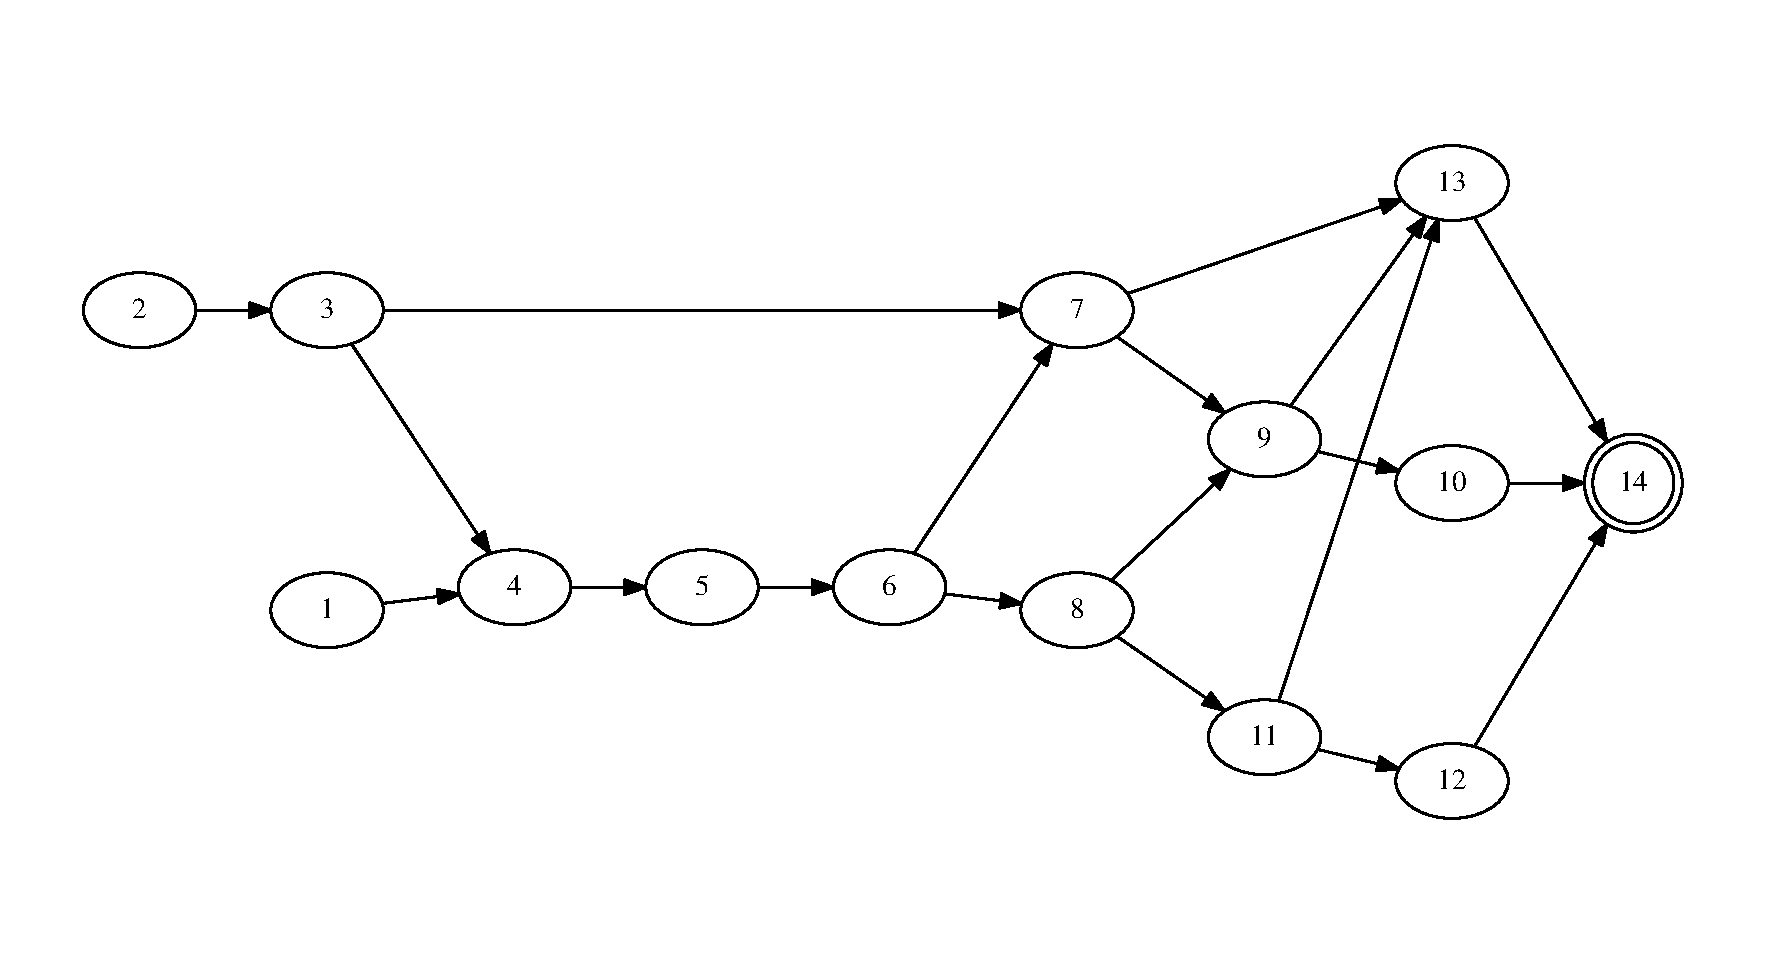
\includegraphics[width=\textwidth]{chapters/preparation/figures/dependencies}
\caption{A directed graph showing which tasks must be completed to begin others. \(A \to B\) shows that \(A\) must be complete before \(B\) may begin.}
\label{fig:requirements-dependencies}
\end{figure}

As far as possible, I followed software engineering good-practice.
All project files were checked into version control (git), and shared (read-only) with supervisors using a well-known hosting website.
Weekly progress meetings were observed to ensure the project did not get off-track.

\section{Starting point}
At the start of the project, I was familiar with the theory required for implementing \(\lambda\)-calculus and type theory.
I was not familiar with approaches to binding described above, or with Isabelle itself.
I am pleased to say I have now learned more about these topics.

\section{Summary}
In this chapter I discussed work that took place before implementation began.
I introduced background theory, covering untyped \(\lambda\)-calculus (\S\ref{sec:lambda-intro}), simple types (\S\ref{sec:type-intro}), \(\alpha\)-equivalence and approaches to this problem (\S\ref{sec:alpha-equivalence}), and introduced nominal techniques (\S\ref{sec:nominal-intro}).
I then described the Isabelle tooling (\S\ref{sec:isabelle-intro}), preparing for practical and theoretical challenges later.
Finally, I decomposed the project into steps (\S\ref{sec:requirements}), and described engineering techniques used to tackle the problem.
